\chapter{Using the Impedance Diagram}
\begin{itemize}
	\item Using impedance diagrams for load flows
	\item Using impedance diagrams for fault calculations
\end{itemize}
\begin{quoting}
	By the end of this synchronous session you should be comfortable with how impedance diagrams can be used to calculate load flows and perform fault calculations in an electrical power system
\end{quoting}
\section{Load Flow Calculation}
\subsection{Load flow}
\begin{itemize}
	\item In an electrical power system currents flow from generators to loads via a transmission/distribution system thereby permitting `load (power) flows'
	\item If a system is at steady-state then currents and power flows would be stable
	\item If there is a change in the system e.g. suddenly and additional load is connected, then there will be a change to currents and load flow
	\item An electrical system cannot change instantaneously from one state to another. The generators for example cannot instantaneously change the supply of power at the point load changes. There will be a transient period
\end{itemize}
\subsection{Load flow analysis example}
\begin{figure}[H]
	\centering
	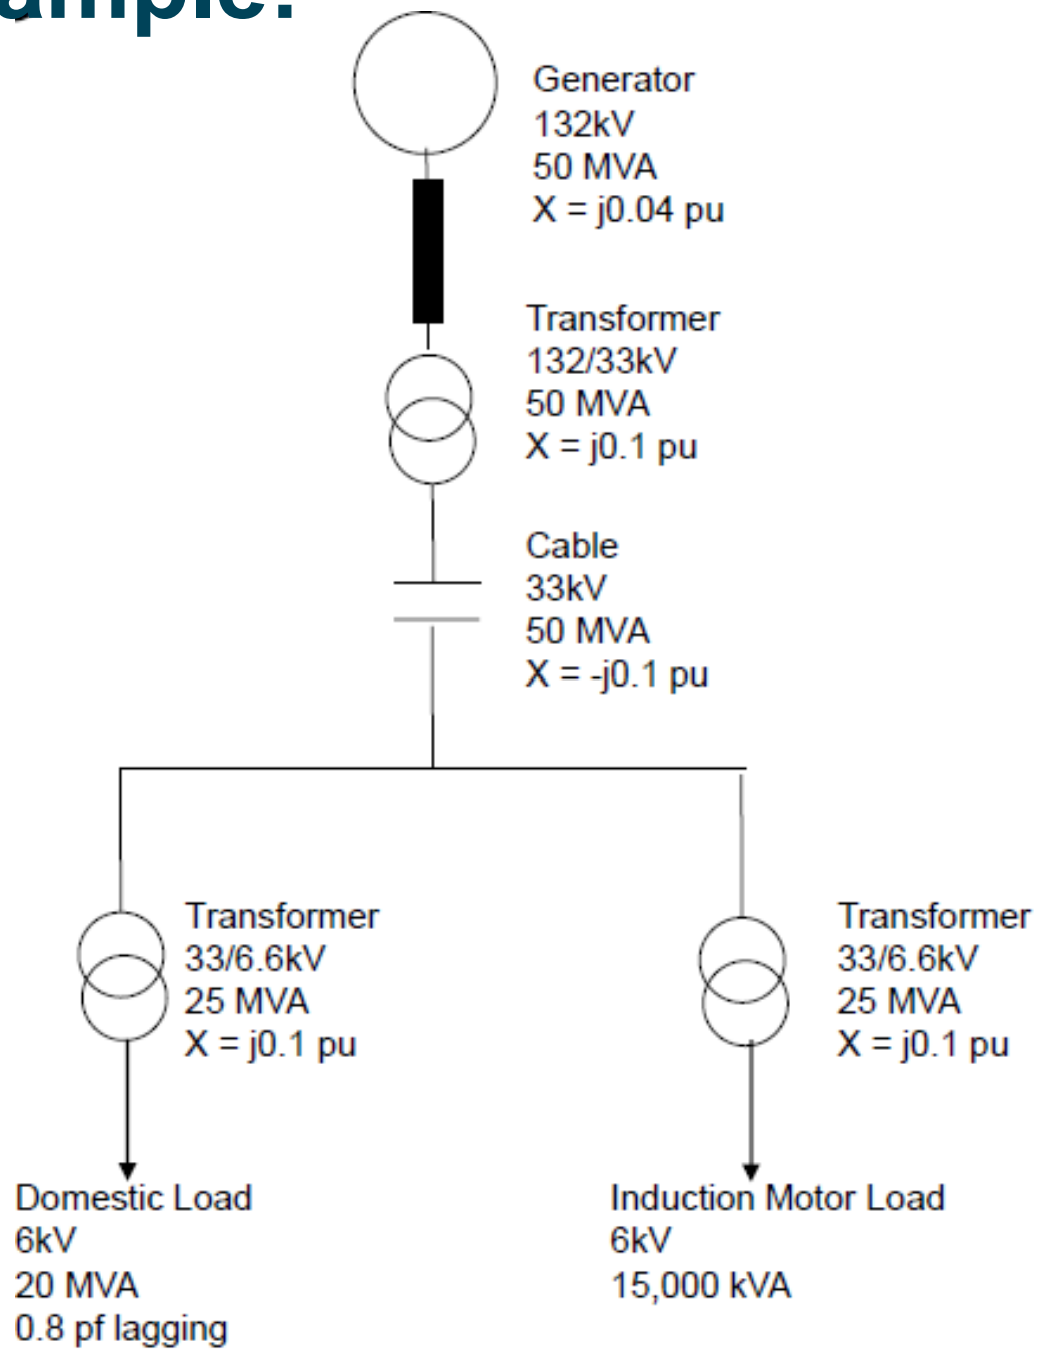
\includegraphics[width = 0.9\textwidth]{./img/figure15.png}
	\caption{Single Line Diagram.}
\end{figure}
A \SI{132}{kV} supply feeds two loads; a group of domestic consumers and a group of induction motors which on starting consume five times rated (or design) full load current at zero power factor lagging.
\subsubsection{Part a}
Convert the single line diagram into an impedance diagram. We will select a base S of \SI{50}{MVA} and \SI{33}{kV} as the base V. The values selected can be different but must be stated by the designer.
\begin{figure}[H]
	\centering
	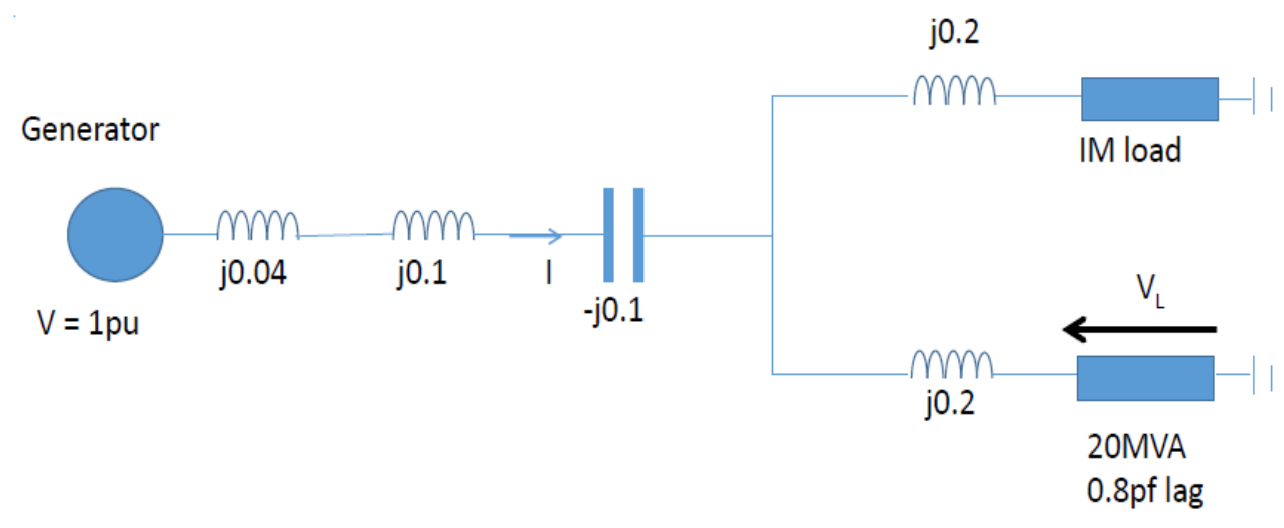
\includegraphics[width =  \textwidth]{./img/figure16.png}
	\caption{Single Line Diagram.}
\end{figure}
Here is the Impedance Diagram of the Single Line Diagram where all the impedances have been changed into per unit values on a \SI{50}{MVA} base.
\subsubsection{Part b}
Calculate the voltage at the domestic busbars prior to induction motor start.
\begin{itemize}
	\item The induction motor load is open circuit so all current flowing from the generator will flow to the domestic load i.e. steady state
	\item To determine the voltage at the domestic busbar prior to the induction motor start then the equation for $V_L = 1 - IZ$ can be used, where:
	      \begin{itemize}
		      \item $V_L$ is the domestic voltage
		      \item 1 is the pu voltage at the generator
		      \item $I$ is the generator current
		      \item $Z$ is the system impedance between source and load
	      \end{itemize}
\end{itemize}
Calculating the impedance of the circuit then:
\begin{gather}
	Z = j\left(0.04 + 0.1 - 0.1 + 0.2\right) = j0.24
\end{gather}
Calculating the current in the circuit then:
\begin{gather}
	I = \frac{20 \times 10^6}{\sqrt{3}\times 6000} = \SI{1925}{A}\textrm{ at 0.8 pf lag}
\end{gather}
Now defining base current related to domestic side (although the domestic side is rated at \SI{6}{kV}, the transformer is rated at \SI{6.6}{kV} and it is permissible to use this values as it is correct in the SLD and ID), we can say:
\begin{gather}
	\textrm{Base current at }\SI{6.6}{kV} = \frac{50\times 10^6}{\sqrt{3}\times 6.6\times 10^3} = \SI{4374}{A}\\
	\textrm{Domestic current pu } = \frac{1925}{4374} = 0.44 \textrm{ at 0.8 pf lag}\\
	V_L' = 1 - j0.04\left[0.44\left(0.8-j0.6\right)\right] - j0.2\left[0.44\left(0.8-j0.6\right)\right] = \SI{0.94}{pu}
\end{gather}
\subsubsection{Part c}
Calculate the maximum voltage dip that will occur when all the induction motors are started together at the same moment in time. The induction motor switch is now closed. The demand at this moment is five times normal full-load current. The induction motor load demands a substantial current:
\begin{gather}
	\textrm{Starting current IM} = -j\frac{15000 \times 10^3}{\sqrt{3}\times 6000}\times 5 = -j7217\,\si{A}\\
	\textrm{Starting current IM} = -j\frac{7217}{4374} = -j1.64\,\si{pu}
\end{gather}
The induction motor load demands a substantial current which flows from the generator. Remember at IM start there is no real power so all power is reactive hence zero power factor. The voltage at the terminals will drop across the series connected devices:
\begin{gather}
	V_L' = 1-j0.04\left[0.44\left(0.8-j0.6\right)-j1.64\right]-j0.2\left[0.44\left(0.8-j0.6\right)\right]\\
	= 0.871 -j0.084 = 0.875\,\si{pu}
\end{gather}
Hence the voltage dips from \SI{0.94}{pu} to \SI{0.87}{pu} or alternatively from \SI{6.204}{kV} to \SI{5.78}{pu}. The voltage dip would be noticed temporarily as a light flicker or dimming. In practice, the generator would recover after a few seconds - transient response of the generator.
\subsection{Some thoughts}
\begin{itemize}
	\item Understand the initial conditions first and then calculate the impact of load changes
	\item The line series capacitor installed has partially neutralised the network inductance. Without this capacitance the dip would be much more severe
	\item Voltage flicker often occurs when there is a sudden demand for large power is demanded e.g. starting of large induction motors on ships or in grids e.g. near steel rolling mills or factories
\end{itemize}
\section{Using impedance diagrams in short-circuit balanced faults}
\subsection{Fault classification}
Faults may be classified as being:
\begin{itemize}
	\item Open circuit faults
	\item Short circuit faults
\end{itemize}
Faults may occur in high voltage and low voltage systems meaning:
\begin{itemize}
	\item Three-phase system faults
	\item Single-phase system faults
	\item DC system faults
\end{itemize}
For short circuit fault types then the engineer needs to appreciate its significance and protect against such events. Faults have two main characteristics: MVA fault level (\si{MVA}) and fault current ($I_{fault}$).
\subsection{Types of faults}
Symmetrical fault (Fault currents are balanced in each phase)
\begin{itemize}
	\item Three-phase short circuit
	\item Three-phase to ground fault
	\item (Three-phase open circuit)
\end{itemize}
Unsymmetrical fault (fault currents are \textbf{not} balanced in each phase)
\begin{itemize}
	\item Single-phase to earth
	\item Double-phase to earth
	\item Two-phases short together
	\item Single-phase open circuit
	\item Double-phase open circuit
\end{itemize}
\subsection{Faults normally are due to:}
\begin{itemize}
	\item Wearing of insulation
	\item Ageing
	\item Poor connections
	\item Fault due to lightning
	\item Tree limbs falling on the line
	\item Wind, weather impacts
	\item Impact/shock damage
	\item Vandalism
	\item Poor safety protocols or work on live equipment
\end{itemize}
\subsection{MVA method}
\begin{itemize}
	\item The MVA method is used to define the power at the point of a fault
	\item The accepted method is to calculate the Fault MVA as follows:
\end{itemize}
\begin{gather}
	MVA_{fault} = \frac{\textrm{Base S (MVA)}}{\textrm{Impedance to fault (pu)}}
\end{gather}
\begin{itemize}
	\item Having calculated the $\si{MVA}_{fault}$ the fault current can be calculated using the nominal voltage at the fault
\end{itemize}
\begin{gather}
	I_{fault} = \frac{\si{MVA}_{fault}}{\sqrt{3}\times V_{base}}
\end{gather}
\subsection{Balanced three-phase fault}
\begin{figure}[H]
	\centering
	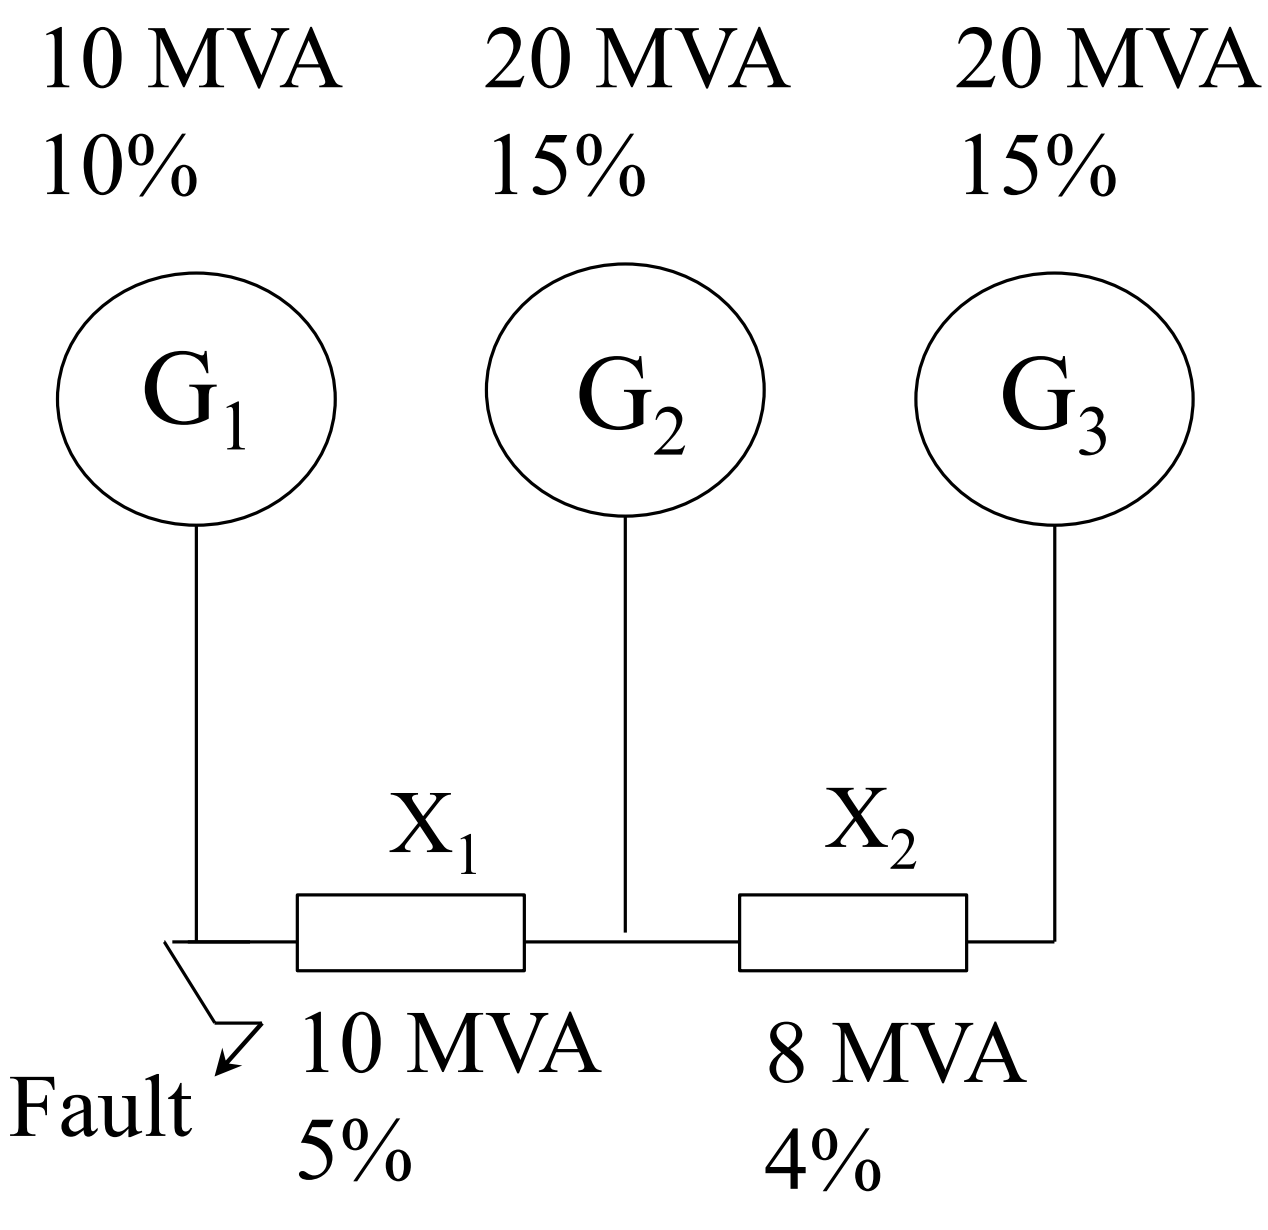
\includegraphics[width = 0.8\textwidth]{./img/figure17.png}
	\caption{Balanced three-phase fault.}
\end{figure}
An interconnected generator-reactor system is active and suddenly incurs a balanced three-phase short circuit at the Fault indicated. Using a \SI{50}{MVA} base then draw an impedance diagram and hence determine the Fault Level and Fault Current. It is an \SI{11}{kV} three phase system.
\subsection{Solution}
\begin{figure}[H]
	\centering
	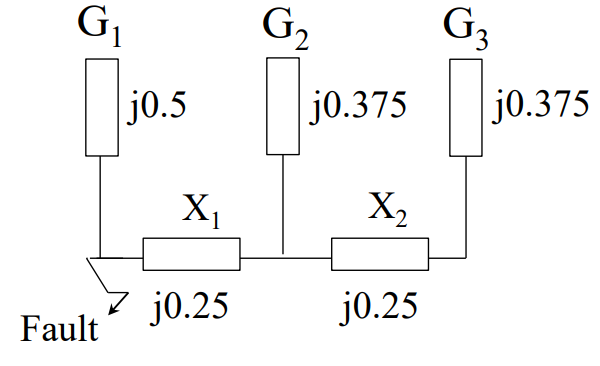
\includegraphics[width = 0.8\textwidth]{./img/figure18.png}
	\caption{Impedance diagram.}
\end{figure}
\begin{gather}
	X_{G1} = \frac{50}{10}\cdot 0.1 = \SI{0.5}{pu}\\
	X_{G2} = \frac{50}{20}\cdot 0.15 = \SI{0.375}{pu}\\
	X_{G3} = \frac{50}{20}\cdot 0.15 = \SI{0.375}{pu}\\
	X_1 = \frac{50}{10}\cdot 0.05 = \SI{0.25}{pu}\\
	X_1 = \frac{50}{8}\cdot 0.04 = \SI{0.25}{pu}
\end{gather}
\begin{figure}[H]
	\centering
	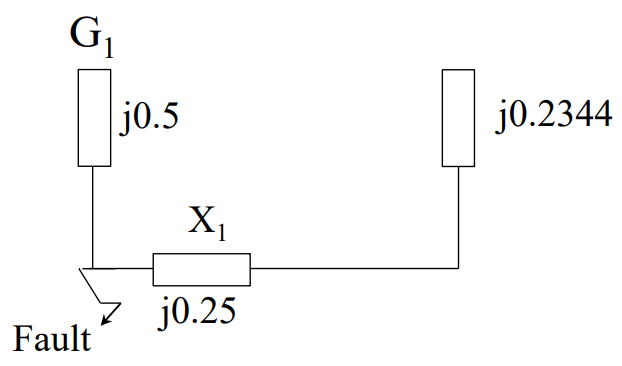
\includegraphics[width = 0.8\textwidth]{./img/figure19.png}
	\caption{Impedance diagram circuit reduced.}
\end{figure}
\begin{gather}
	\textrm{Per unit reactance} = \frac{0.5\left(0.2344 + 0.25\right)}{0.5 + \left(0.2344 + 0.25\right)} = j0.246\\
	\textrm{MVA Fault Level} = \frac{50\times 10^3}{0.246} = \SI{203.25}{MVA}\\
	\textrm{Fault current} = \frac{203.25 \times 10^6}{\sqrt{3}\times 11\times 10^3} = \SI{10668}{A}
\end{gather}
The MVA Fault Level provides information on the `power at the fault'. The Fault Current provides information on protection e.g. circuit breakers. This is known as the symmetrical fault current.
\subsection{Importance of MVA}
\begin{itemize}
	\item The short circuit capacity (SCC) at the busbar is the fault level of the busbar. The strength of a busbar (or the ability to maintain its voltage) is directly proportional to its SCC.
	\item An infinitely strong bus (or infinite bus bar) has an infinite SCC, with a zero equivalent impedance and will maintain its voltage under all conditions
	\item Magnitude of short circuit current is time dependent due to synchronous generators. It is initially at its largest value and decreasing to steady value. These higher fault levels tax circuit breakers (CB) adversely so that current limiting reactors are sometimes used
\end{itemize}
\subsection{Power system symmetrical faults}
\begin{itemize}
	\item In a power system, knowing the maximum MVA Fault Level and the Fault Current that could potentially flow into a zero impedance fault is necessary in order to rate switch gear correctly
	\item The MVA Fault Level defines the maximum MVA that is experience when a symmetrical fault event occurs. The fault level is usually expressed in MVA (or a corresponding per-unit value)
	\item The maximum fault current can be calculated using the MVA Fault Level and the nominal Voltage Rating at the fault location
\end{itemize}
\subsection{Conclusions}
\begin{itemize}
	\item The analysis show in this session has explained how impedance diagrams can be used for system analysis for `load flows' and `balanced faults'
	\item For larger or complex circuits then many more calculations are needed meaning computers are generally used to calculate load flows and faults
	\item Various computer programmes are available including MATLAB, Simulink Simpower Systems, PSCAD, ERACS, etc
\end{itemize}













